%%%%%%%%%%%%%%%%%%%%%%%%%%%%%%%%%%%%%%%%%%%%%%%%%%%%%%
% AI History Presentation Template                   %
% Author: Guang Cheng                                %
% UCLA Statistics and Data Science                   %
% Date: \today                                       %
%%%%%%%%%%%%%%%%%%%%%%%%%%%%%%%%%%%%%%%%%%%%%%%%%%%%%%

\documentclass{beamer}
\usepackage{hyperref}
\usepackage[T1]{fontenc}
\usepackage{amssymb}
\usepackage{latexsym,amsmath,xcolor,multicol,booktabs,calligra}
\usepackage{graphicx,pstricks,listings,stackengine}
\usepackage{tikz}

% Standard Colors
\definecolor{MyBlue}{RGB}{0,102,204}
\definecolor{MyLightBlue}{RGB}{173,216,230}
\definecolor{MyDarkBlue}{RGB}{0,51,102}
\definecolor{MyGold}{RGB}{255,215,0}

% Set theme colors
\setbeamercolor{structure}{fg=MyBlue}
\setbeamercolor{frametitle}{fg=MyDarkBlue,bg=MyLightBlue}
\setbeamercolor{title}{fg=MyDarkBlue}
\setbeamercolor{author}{fg=MyBlue}
\setbeamercolor{institute}{fg=MyBlue}
\setbeamercolor{date}{fg=MyBlue}

\author{Guang Cheng \\ Graduate Vice Chair \\ Director of Trustworthy AI Lab \\ Professor of Statistics and Data Science}
\title{The Evolution of Artificial Intelligence}
\subtitle{From Ancient Dreams to Modern Reality}
\institute{University of California, Los Angeles}
\date{\today}

\begin{document}

% Title slide
\begin{frame}
    \titlepage
\end{frame}

% Table of contents
\begin{frame}
    \frametitle{Outline}
    \tableofcontents
\end{frame}

\section{Introduction to Artificial Intelligence}

\begin{frame}
    \frametitle{What is Artificial Intelligence?}
    \begin{block}{Definition}
        \textbf{Artificial Intelligence (AI):} The simulation of human intelligence processes by machines, including learning, reasoning, problem-solving, perception, and language understanding.
    \end{block}
    
    \begin{columns}
        \begin{column}{0.48\textwidth}
            \begin{alertblock}{Narrow AI (Weak AI)}
                \begin{itemize}
                    \item Designed for specific tasks
                    \item Current state of technology
                    \item Examples: voice assistants, recommendation systems, chess programs
                \end{itemize}
            \end{alertblock}
        \end{column}
        \begin{column}{0.48\textwidth}
            \begin{exampleblock}{Artificial General Intelligence}
                \begin{itemize}
                    \item Human-level cognitive abilities
                    \item Adaptable to any intellectual task
                    \item Currently hypothetical
                    \item Timeline: decades to centuries
                \end{itemize}
            \end{exampleblock}
        \end{column}
    \end{columns}
\end{frame}

\begin{frame}
    \frametitle{Historical Timeline Overview}
    \begin{figure}
        \centering
        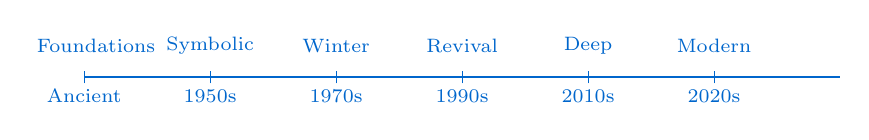
\begin{tikzpicture}[scale=0.8]
            \draw[thick,MyBlue] (0,0) -- (12,0);
            \foreach \x/\year/\label in {0/Ancient/Foundations, 2/1950s/Symbolic, 4/1970s/Winter, 6/1990s/Revival, 8/2010s/Deep, 10/2020s/Modern} {
                \draw[MyBlue] (\x,-0.1) -- (\x,0.1);
                \node[MyBlue] at (\x,-0.3) {\scriptsize \year};
                \node[MyBlue,text width=1.2cm,align=center] at (\x,0.5) {\scriptsize \label};
            }
        \end{tikzpicture}
        \caption{Major Eras in AI Development}
    \end{figure}
    
    \begin{itemize}
        \item \textcolor{MyBlue}{\textbf{Foundations (Ancient-1950s):}} Philosophical groundwork and mathematical foundations
        \item \textcolor{MyBlue}{\textbf{Symbolic AI (1950s-1970s):}} Logic-based systems and early optimism
        \item \textcolor{MyBlue}{\textbf{AI Winters (1970s-1990s):}} Funding cuts and technical limitations
        \item \textcolor{MyBlue}{\textbf{Revival (1990s-2000s):}} Statistical methods and big data
        \item \textcolor{MyBlue}{\textbf{Modern Era (2010s-Present):}} Deep learning and generative AI
    \end{itemize}
\end{frame}

\section{Foundations and Early History}

\begin{frame}
    \frametitle{Ancient Dreams of Artificial Beings}
    \begin{columns}
        \begin{column}{0.48\textwidth}
            \begin{block}{Greek Mythology}
                \begin{itemize}
                    \item \textbf{Hephaestus' Golden Servants:} Mechanical helpers made of gold
                    \item \textbf{Talos of Crete:} Bronze giant guardian 
                    \item \textbf{Pygmalion's Galatea:} Sculpture brought to life
                \end{itemize}
            \end{block}
            
            \begin{block}{Medieval Legends}
                \begin{itemize}
                    \item \textbf{Jewish Golems:} Clay creatures animated by mystical means
                    \item \textbf{Prague Golem:} Most famous 16th century legend
                \end{itemize}
            \end{block}
        \end{column}
        \begin{column}{0.48\textwidth}
            \begin{alertblock}{Early Mechanical Devices}
                \begin{itemize}
                    \item \textbf{Mechanical Clocks (13th-14th c.):} First programmable machines
                    \item \textbf{Leonardo's Robot Knight (1495):} Mechanical suit of armor
                    \item \textbf{Automata:} Self-operating machines
                \end{itemize}
            \end{alertblock}
            
            \begin{exampleblock}{Key Insight}
                Throughout history, humans have imagined creating artificial beings with intelligence and agency.
            \end{exampleblock}
        \end{column}
    \end{columns}
\end{frame}

\begin{frame}
    \frametitle{Philosophical Foundations}
    \begin{columns}
        \begin{column}{0.48\textwidth}
            \begin{block}{Mind and Mechanism}
                \textbf{René Descartes (1596-1650)}
                \begin{itemize}
                    \item Distinguished mind from body
                    \item Animals as complex machines
                    \item Humans have souls, machines don't
                \end{itemize}
                
                \textbf{Thomas Hobbes (1588-1679)}
                \begin{itemize}
                    \item ``Reasoning is but reckoning''
                    \item Thinking could be mechanical computation
                \end{itemize}
            \end{block}
        \end{column}
        \begin{column}{0.48\textwidth}
            \begin{alertblock}{Computational Vision}
                \textbf{Gottfried Leibniz (1646-1716)}
                \begin{itemize}
                    \item Proposed ``calculus ratiocinator''
                    \item Universal symbolic language for reasoning
                    \item Mathematical approach to logic
                \end{itemize}
            \end{alertblock}
            
            \begin{exampleblock}{Central Question}
                \textit{``What if machines could think like humans?''}
            \end{exampleblock}
        \end{column}
    \end{columns}
\end{frame}

\begin{frame}
    \frametitle{Mechanical Computation Era}
    \begin{columns}
        \begin{column}{0.48\textwidth}
            \begin{block}{Charles Babbage (1791-1871)}
                \textbf{The Difference Engine (1822)}
                \begin{itemize}
                    \item Mechanical calculator
                    \item Polynomial functions
                \end{itemize}
                
                \textbf{The Analytical Engine (1837)}
                \begin{itemize}
                    \item First general-purpose computer design
                    \item Had ``mill'' (CPU) and ``store'' (memory)
                    \item Programmable with punched cards
                \end{itemize}
            \end{block}
        \end{column}
        \begin{column}{0.48\textwidth}
            \begin{alertblock}{Ada Lovelace (1815-1852)}
                \textbf{World's First Programmer}
                \begin{itemize}
                    \item Wrote first computer algorithm
                    \item Envisioned creative potential
                    \item ``Machines might compose elaborate music''
                \end{itemize}
            \end{alertblock}
            
            \begin{exampleblock}{Revolutionary Insight}
                Machines could manipulate symbols and follow complex instructions, not just arithmetic.
            \end{exampleblock}
        \end{column}
    \end{columns}
\end{frame}

\begin{frame}
    \frametitle{Mathematical Foundations (1930s-1940s)}
    \begin{columns}
        \begin{column}{0.48\textwidth}
            \begin{block}{Kurt Gödel (1906-1978)}
                \textbf{Incompleteness Theorems (1931):}
                \begin{itemize}
                    \item Any complex logical system contains unprovable statements
                    \item No system can prove its own consistency
                    \item Showed fundamental limits to formal systems
                    \item Influenced later thinking about AI limitations
                \end{itemize}
            \end{block}
        \end{column}
        \begin{column}{0.48\textwidth}
            \begin{block}{Alan Turing (1912-1954)}
                \textbf{``On Computable Numbers'' (1936):}
                \begin{itemize}
                    \item Defined algorithmic computation
                    \item Turing Machine theoretical model
                    \item Established limits of computation
                    \item Church-Turing Thesis
                \end{itemize}
            \end{block}
        \end{column}
    \end{columns}
    
    \begin{exampleblock}{Key Insight}
        These mathematicians established the theoretical foundations for understanding what it means to compute and think algorithmically.
    \end{exampleblock}
\end{frame}

\begin{frame}
    \frametitle{The Turing Test (1950)}
    \begin{block}{Alan Turing's ``Computing Machinery and Intelligence''}
        \textbf{Central Question:} ``Can machines think?''
        
        Turing proposed the \textbf{Imitation Game} as a practical test:
    \end{block}
    
    \begin{center}
        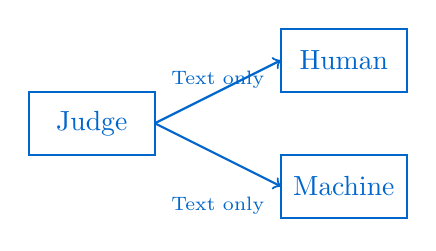
\begin{tikzpicture}[scale=0.8]
            \draw[MyBlue,thick] (0,2) rectangle (2,3) node[pos=.5] {Judge};
            \draw[MyBlue,thick] (4,3) rectangle (6,4) node[pos=.5] {Human};
            \draw[MyBlue,thick] (4,1) rectangle (6,2) node[pos=.5] {Machine};
            \draw[MyBlue,thick,->] (2,2.5) -- (4,3.5);
            \draw[MyBlue,thick,->] (2,2.5) -- (4,1.5);
            \node[MyBlue] at (3,3.2) {\scriptsize Text only};
            \node[MyBlue] at (3,1.2) {\scriptsize Text only};
        \end{tikzpicture}
    \end{center}
    
    \begin{alertblock}{Test Criteria}
        If the judge cannot reliably distinguish between human and machine responses, the machine \textbf{passes the test}.
    \end{alertblock}
    
    \textcolor{MyBlue}{\textbf{Paradigm Shift:}} Focus on observable behavior rather than internal processes.
\end{frame}

\section{The Birth and Early Development of AI}

\begin{frame}
    \frametitle{The Dartmouth Workshop (1956)}
    \begin{block}{Birth of Artificial Intelligence}
        \textbf{John McCarthy} coined the term ``Artificial Intelligence'' for the Dartmouth Summer Research Project.
    \end{block}
    
    \begin{columns}
        \begin{column}{0.48\textwidth}
            \begin{alertblock}{Key Participants}
                \begin{itemize}
                    \item \textbf{Allen Newell} - Logic Theorist
                    \item \textbf{Herbert Simon} - Nobel laureate
                    \item \textbf{Claude Shannon} - Information theory
                \end{itemize}
            \end{alertblock}
        \end{column}
        \begin{column}{0.48\textwidth}
            \begin{exampleblock}{Research Objectives}
                \begin{itemize}
                    \item Make machines use language
                    \item Solve human-reserved problems
                    \item Improve themselves automatically
                \end{itemize}
            \end{exampleblock}
        \end{column}
    \end{columns}
    
    \begin{block}{Historic Achievement}
        AI established as a legitimate scientific field with concrete research goals.
    \end{block}
\end{frame}

\begin{frame}
    \frametitle{Symbolic AI Era (1950s-1960s)}
    \begin{columns}
        \begin{column}{0.48\textwidth}
            \begin{block}{Logic Theorist (1956)}
                \textbf{Creators:} Newell \& Simon
                \begin{itemize}
                    \item First AI program to prove theorems
                    \item Proved 38 of 52 theorems in Principia Mathematica
                    \item One proof more elegant than original
                \end{itemize}
            \end{block}
            
            \begin{block}{General Problem Solver}
                \textbf{Method:} Means-ends analysis
                \begin{itemize}
                    \item Compare current to goal state
                    \item Find operations to reduce differences
                \end{itemize}
            \end{block}
        \end{column}
        \begin{column}{0.48\textwidth}
            \begin{alertblock}{Core Philosophy}
                
                \textbf{Intelligence = Logic + Symbol Manipulation}
                
            \end{alertblock}
            
            \begin{exampleblock}{Algorithm Example}
                \texttt{Problem:} Move blocks A, B, C
                
                \texttt{Rules:} IF block X on Y AND goal X on table THEN remove X from Y
                
                \texttt{Method:} Apply rules systematically
            \end{exampleblock}
        \end{column}
    \end{columns}
\end{frame}

\section{Neural Networks and Expert Systems}

\begin{frame}
    \frametitle{Early Neural Networks (1960s)}
    \begin{block}{Frank Rosenblatt's Perceptron (1957)}
        \textbf{Inspiration:} Biological neurons in the brain
        
        \textbf{Algorithm:}
        \begin{align}
            \text{Input:} \quad &x_1, x_2, x_3, \ldots \text{ (features)} \\
            \text{Weights:} \quad &w_1, w_2, w_3, \ldots \text{ (learned)} \\
            \text{Output:} \quad &f(w_1x_1 + w_2x_2 + w_3x_3 + \text{bias})
        \end{align}
    \end{block}
    
    \begin{alertblock}{The Perceptron Controversy (1969)}
        \textbf{Minsky \& Papert's critique revealed limitations:}
        \begin{itemize}
            \item Cannot solve XOR problem (non-linearly separable)
            \item Limited to linear decision boundaries
            \item Multi-layer networks computationally intractable
        \end{itemize}
        
        \textcolor{red}{\textbf{Impact:}} Neural network research funding dried up for 20 years.
    \end{alertblock}
\end{frame}

\begin{frame}
    \frametitle{Expert Systems Revolution (1970s)}
    \begin{columns}
        \begin{column}{0.48\textwidth}
            \begin{block}{DENDRAL (1965-1970s)}
                \textbf{Purpose:} Chemical analysis
                \begin{itemize}
                    \item Molecular structure identification
                    \item First successful expert system
                    \item Knowledge base + inference engine
                \end{itemize}
            \end{block}
            
            \begin{exampleblock}{Rule Example}
                \texttt{IF:} Patient has fever AND bacteria culture is gram-positive
                
                \texttt{THEN:} Evidence (0.7) organism is streptococcus
            \end{exampleblock}
        \end{column}
        \begin{column}{0.48\textwidth}
            \begin{block}{MYCIN (1970s)}
                \textbf{Purpose:} Medical diagnosis
                \begin{itemize}
                    \item Blood infection treatment
                    \item Often outperformed doctors
                    \item 600+ IF-THEN rules
                    \item Handled uncertainty
                \end{itemize}
            \end{block}
            
            \begin{alertblock}{Success Formula}
                \begin{center}
                    Domain Expertise + Rules + Uncertainty = Practical AI
                \end{center}
            \end{alertblock}
        \end{column}
    \end{columns}
\end{frame}

\section{AI Winters and Revival}

\begin{frame}
    \frametitle{The First AI Winter (1974-1980)}
    \begin{alertblock}{What Went Wrong?}
        \begin{columns}
            \begin{column}{0.48\textwidth}
                \textbf{Overpromising:}
                \begin{itemize}
                    \item Herbert Simon (1957): ``Within 10 years a computer will be chess champion''
                    \item Marvin Minsky (1967): ``Within a generation... AI will be solved''
                    \item Reality: Systems remained narrow and brittle
                \end{itemize}
            \end{column}
            \begin{column}{0.48\textwidth}
                \textbf{Technical Limitations:}
                \begin{itemize}
                    \item Combinatorial explosion
                    \item Limited computational power
                    \item Lack of common sense
                    \item Real-world complexity
                \end{itemize}
            \end{column}
        \end{columns}
    \end{alertblock}
    
    \begin{center}
        \textcolor{MyBlue}{\textbf{\Large 50\% Funding Reduction}}
    \end{center}
    
    \begin{block}{The Lighthill Report (1973)}
        UK government assessment criticized AI research for failing to achieve goals, leading to massive funding cuts.
    \end{block}
\end{frame}

\begin{frame}
    \frametitle{Commercial AI Boom (1980s)}
    \begin{block}{XCON (Expert Configurer)}
        \textbf{Company:} Digital Equipment Corporation
        \begin{itemize}
            \item Configured complex computer systems
            \item Saved \$25 million annually
            \item 2,500 rules, 80,000 orders/year by 1986
        \end{itemize}
    \end{block}
    
    \begin{columns}
        \begin{column}{0.48\textwidth}
            \begin{exampleblock}{Industry Applications}
                \begin{itemize}
                    \item \textbf{Finance:} Credit approval, fraud detection
                    \item \textbf{Manufacturing:} Quality control
                    \item \textbf{Telecom:} Network diagnostics
                \end{itemize}
            \end{exampleblock}
        \end{column}
        \begin{column}{0.48\textwidth}
            \begin{alertblock}{Market Growth}
                
                \textbf{\$2 Billion} AI industry revenue by 1988
                
                \begin{itemize}
                    \item Hundreds of AI companies founded
                    \item Major corporate investments
                \end{itemize}
            \end{alertblock}  
        \end{column}
    \end{columns}
    
    \textcolor{MyBlue}{\textbf{Paradigm Shift:}} AI moved from academic research to commercial reality.
\end{frame}

\begin{frame}
    \frametitle{The Second AI Winter (Late 1980s-1990s)}
    \begin{alertblock}{A Deeper Freeze}
        \begin{columns}
            \begin{column}{0.48\textwidth}
                \textbf{Expert System Brittleness:}
                \begin{itemize}
                    \item Broke with unexpected inputs
                    \item Expensive to maintain
                    \item Knowledge acquisition bottleneck
                    \item Couldn't learn or adapt
                \end{itemize}
            \end{column}
            \begin{column}{0.48\textwidth}
                \textbf{Economic Factors:}
                \begin{itemize}
                    \item Specialized hardware obsolete
                    \item PCs offered better value
                    \item Economic recession
                    \item Venture capital fled AI
                \end{itemize}
            \end{column}
        \end{columns}
    \end{alertblock}
    
    \begin{center}
        \textcolor{red}{\textbf{\Large 70\% Decline in VC Investment (1987-1991)}}
    \end{center}
    
    \begin{exampleblock}{Silver Lining}
        The winter forced researchers to focus on fundamental problems and develop more robust approaches.
    \end{exampleblock}
\end{frame}

\section{Machine Learning Revival and Modern AI}

\begin{frame}
    \frametitle{Machine Learning Revival (1990s)}
    \begin{block}{Paradigm Shift: From Rules to Data}
        \begin{center}
            \textbf{Hand-coded Rules} $\rightarrow$ \textbf{Learning from Data}
        \end{center}
    \end{block}
    
    \begin{columns}
        \begin{column}{0.33\textwidth}
            \begin{alertblock}{Decision Trees}
                \begin{itemize}
                    \item Interpretable
                    \item ID3/C4.5 algorithms
                    \item Random Forests
                    \item Ensemble methods
                \end{itemize}
            \end{alertblock}
        \end{column}
        \begin{column}{0.33\textwidth}
            \begin{exampleblock}{Support Vector Machines}
                \begin{itemize}
                    \item Maximum margin
                    \item Kernel trick
                    \item Non-linear problems
                    \item Excellent performance
                \end{itemize}
            \end{exampleblock}
        \end{column}
        \begin{column}{0.33\textwidth}
            \begin{block}{Bayesian Networks}
                \begin{itemize}
                    \item Probabilistic reasoning
                    \item Handle uncertainty
                    \item Medical diagnosis
                    \item Principled approach
                \end{itemize}
            \end{block}
        \end{column}
    \end{columns}
    
    \begin{block}{Mathematical Formulation (SVM)}
        Find hyperplane maximizing margin: $w \cdot x + b = 0$
        
        Kernel functions: $K(x,y) = \phi(x) \cdot \phi(y)$ for non-linear mapping
    \end{block}
\end{frame}

\begin{frame}
    \frametitle{Deep Learning Renaissance (2006-2012)}
    \begin{block}{Geoffrey Hinton's Breakthrough (2006)}
        \textbf{Deep Belief Networks:} Multi-layer neural networks with unsupervised pre-training
        
        \textbf{Innovation:} Layer-by-layer training overcame vanishing gradient problem
    \end{block}
    
    \begin{columns}
        \begin{column}{0.48\textwidth}
            \begin{alertblock}{Training Process}
                \begin{enumerate}
                    \item Unsupervised pre-training
                    \item Supervised fine-tuning
                    \item Backpropagation optimization
                    \item Regularization (dropout)
                \end{enumerate}
            \end{alertblock}
        \end{column}
        \begin{column}{0.48\textwidth}
            \begin{exampleblock}{Technical Breakthroughs}
                \begin{itemize}
                    \item Restricted Boltzmann Machines
                    \item Contrastive Divergence algorithm
                    \item GPU acceleration
                    \item ReLU activation functions
                \end{itemize}
            \end{exampleblock}
        \end{column}
    \end{columns}
    
    \begin{alertblock}{ImageNet Revolution (2012)}
        \textbf{AlexNet:} 8-layer CNN by Krizhevsky, Sutskever, Hinton
        
        \textbf{Performance:} 15.3\% vs 26.2\% error rate - \textbf{10.8\% improvement!}
    \end{alertblock}
\end{frame}

\section{Recent Breakthroughs and Current Challenges}

\begin{frame}
    \frametitle{Transformer Revolution (2017-2020)}
    \begin{block}{``Attention Is All You Need'' (Vaswani et al., 2017)}
        \textbf{Innovation:} Self-attention mechanism replaced recurrence
        
        \textbf{Mathematical Foundation:}
        $$\text{Attention}(Q,K,V) = \text{softmax}\left(\frac{QK^T}{\sqrt{d_k}}\right)V$$
    \end{block}
    
    \begin{columns}
        \begin{column}{0.48\textwidth}
            \begin{alertblock}{BERT (2018)}
                \textbf{Bidirectional Encoder}
                \begin{itemize}
                    \item Masked language modeling
                    \item Bidirectional context
                    \item Fine-tuned for tasks
                    \item SOTA on 11 NLP benchmarks
                \end{itemize}
            \end{alertblock}
        \end{column}
        \begin{column}{0.48\textwidth}
            \begin{exampleblock}{GPT Series (2018-2020)}
                \textbf{Generative Pre-training}
                \begin{itemize}
                    \item GPT-1: 117M parameters
                    \item GPT-2: 1.5B parameters
                    \item GPT-3: 175B parameters
                    \item Emergent abilities with scale
                \end{itemize}
            \end{exampleblock}
        \end{column}
    \end{columns}
    
    \textcolor{MyBlue}{\textbf{Scaling Laws:}} Larger models + more data + more compute = dramatically better performance
\end{frame}

\begin{frame}
    \frametitle{Generative AI Era (2021-Present)}
    \begin{alertblock}{The ChatGPT Phenomenon}
        \begin{center}
            \textbf{100 Million Users in 2 Months}
        \end{center}
        \begin{itemize}
            \item Conversational AI mainstream adoption
            \item Instruction-following and helpfulness
            \item Reinforcement Learning from Human Feedback (RLHF)
            \item Sparked global AI transformation
        \end{itemize}
    \end{alertblock}
\end{frame}  

\begin{frame}
    \frametitle{Generative AI Era (2021-Present)}
    \begin{columns}
        \begin{column}{0.48\textwidth}
            \begin{block}{Multimodal Capabilities}
                \begin{itemize}
                    \item \textbf{DALL-E 2:} Text-to-image
                    \item \textbf{GPT-4V:} Vision-language
                    \item \textbf{Whisper:} Speech recognition
                    \item \textbf{Codex:} Code generation
                \end{itemize}
            \end{block}
        \end{column}
        \begin{column}{0.48\textwidth}
            \begin{exampleblock}{Creative Applications}
                \begin{itemize}
                    \item Art generation (Midjourney, Stable Diffusion)
                    \item Writing assistance and content creation
                    \item Music composition (AIVA)
                    \item Video generation (Runway ML)
                \end{itemize}
            \end{exampleblock}
        \end{column}
    \end{columns}
    
    \begin{center}
        \textcolor{MyBlue}{\textbf{\$100+ Billion}} invested in generative AI startups in 2023
    \end{center}
\end{frame}

\section{Current Challenges and Future Directions}

\begin{frame}
    \frametitle{Critical Challenges in Modern AI}
    
        \begin{column}{0.48\textwidth}
            \begin{alertblock}{Ethics and Bias}
                \begin{itemize}
                    \item \textbf{Algorithmic Bias:} Unfair treatment of minorities
                    \item \textbf{Training Data Issues:} Historical biases embedded
                    \item \textbf{Fairness Metrics:} Measuring and ensuring equity
                    \item \textbf{Transparency:} ``Black box'' decision making
                \end{itemize}
            \end{alertblock}
        \end{column}
        \begin{column}{0.48\textwidth}
            \begin{block}{AI Safety and Alignment}
                \begin{itemize}
                    \item \textbf{Control Problem:} Ensuring desired behavior
                    \item \textbf{Value Alignment:} Matching human values
                    \item \textbf{Existential Risk:} Superintelligent AI dangers
                    \item \textbf{Robustness:} Unexpected situation handling
                \end{itemize}
            \end{block}
        \end{column}

\end{frame}

\begin{frame}
    \frametitle{Critical Challenges in Modern AI}
        
        \begin{column}{0.48\textwidth}
            \begin{exampleblock}{Regulation and Governance}
                \begin{itemize}
                    \item \textbf{EU AI Act:} Comprehensive regulation framework
                    \item \textbf{US Executive Orders:} Federal oversight initiatives
                    \item \textbf{International Cooperation:} Global governance challenges
                    \item \textbf{Industry Standards:} Self vs. mandatory regulation
                \end{itemize}
            \end{exampleblock}
        \end{column}
        \begin{column}{0.48\textwidth}
            \begin{alertblock}{Economic and Social Impact}
                \begin{itemize}
                    \item \textbf{Job Displacement:} Knowledge work automation
                    \item \textbf{Economic Inequality:} Benefit concentration
                    \item \textbf{Education Transformation:} Curriculum adaptation
                    \item \textbf{Privacy Concerns:} Data collection and surveillance
                \end{itemize}
            \end{alertblock}
        \end{column}   
    \begin{center}
        \textcolor{red}{\textbf{50\%}} of jobs could be significantly impacted by AI in next 20 years
    \end{center}
    
\end{frame}

\begin{frame}
    \frametitle{The Path Forward: Trustworthy AI}
    \begin{block}{Trustworthy AI Principles}
        \begin{columns}
            \begin{column}{0.48\textwidth}
                \textbf{Technical Requirements:}
                \begin{itemize}
                    \item \textbf{Robustness:} Reliable performance
                    \item \textbf{Explainability:} Interpretable decisions
                    \item \textbf{Fairness:} Unbiased outcomes
                    \item \textbf{Privacy:} Data protection
                \end{itemize}
            \end{column}
            \begin{column}{0.48\textwidth}
                \textbf{Governance Requirements:}
                \begin{itemize}
                    \item \textbf{Accountability:} Clear responsibility
                    \item \textbf{Transparency:} Open processes
                    \item \textbf{Human Oversight:} Meaningful control
                    \item \textbf{Sustainability:} Environmental consideration
                \end{itemize}
            \end{column}
        \end{columns}
    \end{block}

\end{frame}

\begin{frame}
    \frametitle{The Path Forward: Trustworthy AI}

    \begin{alertblock}{Trustworthy AI Lab Focus Areas}
        \begin{itemize}
            \item \textbf{Statistical Foundations:} Rigorous mathematical frameworks for AI reliability
            \item \textbf{Causal Inference:} Understanding cause-effect relationships in AI systems
            \item \textbf{Uncertainty Quantification:} Measuring and communicating AI confidence
            \item \textbf{Algorithmic Fairness:} Developing bias-free machine learning methods
            \item \textbf{Robust Statistics:} AI systems resilient to data corruption and adversarial attacks
        \end{itemize}
    \end{alertblock}
    
\end{frame}

\section{Conclusion}

\begin{frame}
    \frametitle{Key Lessons from AI History}
    \begin{alertblock}{Cyclical Nature of Progress}
        \begin{itemize}
            \item \textbf{Hype Cycles:} Periods of excitement followed by disappointment
            \item \textbf{Technical Reality:} Progress often slower than initial predictions
            \item \textbf{Breakthrough Moments:} Sudden advances reshape the field
            \item \textbf{Persistence Pays:} Long-term research investments crucial
        \end{itemize}
    \end{alertblock}

\end{frame}

\begin{frame}
    \frametitle{Key Lessons from AI History}
    \begin{columns}
        \begin{column}{0.48\textwidth}
            \begin{block}{Success Factors}
                \begin{itemize}
                    \item \textbf{Interdisciplinary Approach:} Math, CS, Psychology, Philosophy
                    \item \textbf{Hardware-Software Synergy:} Computational advances enable AI
                    \item \textbf{Data-Driven Methods:} More data often beats better algorithms
                    \item \textbf{Open Research:} Collaboration accelerates progress
                \end{itemize}
            \end{block}
        \end{column}
        \begin{column}{0.48\textwidth}
            \begin{exampleblock}{Ongoing Challenges}
                \begin{itemize}
                    \item \textbf{Ethical Considerations:} Every generation must address AI's impact
                    \item \textbf{Technical Limitations:} Fundamental problems remain unsolved
                    \item \textbf{Societal Integration:} Balancing benefits and risks
                    \item \textbf{Global Cooperation:} International coordination needed
                \end{itemize}
            \end{exampleblock}
        \end{column}
    \end{columns}
    
    \begin{center}
        \textcolor{MyBlue}{\textbf{The future of AI depends on our choices today}}
    \end{center}
\end{frame}

%%%
%\begin{frame}
%    \frametitle{The Road Ahead: Research Priorities}
%    \begin{block}{Technical Research Priorities}
%        \begin{columns}
%            \begin{column}{0.48\textwidth}
%               \textbf{Foundational Research:}
%               \begin{itemize}
%                    \item Mathematical theory of intelligence
%                    \item Causal reasoning and inference
%                    \item Few-shot and meta-learning
%                    \item Continual and lifelong learning
%                    \item Compositional and systematic generalization
%                \end{itemize}
%            \end{column}
%            \begin{column}{0.48\textwidth}
%                \textbf{Applied Research:}
%                \begin{itemize}
%                    \item Multimodal and embodied AI
%                    \item Human-AI interaction design
%                    \item AI for scientific discovery
%                    \item Sustainable and efficient AI
%                    \item Domain-specific AI applications
%                \end{itemize}
%            \end{column}
%        \end{columns}
%    \end{block}
    
%    \begin{alertblock}{Trustworthy AI Research}
%        \textbf{Mission:} Develop statistical foundations and methodological frameworks for reliable, fair, and interpretable AI systems that benefit society.
        
%        \textbf{Key Areas:} Robust statistics, causal inference, uncertainty quantification, algorithmic fairness, and AI safety.
%    \end{alertblock}
    
%    \begin{exampleblock}{Call to Action}
%        The next chapter of AI history is being written now. Join us in building AI systems that are not just powerful, but trustworthy and beneficial for all.
%    \end{exampleblock}
%\end{frame}
%%%

\begin{frame}
    \frametitle{Thank You}
    \begin{center}
        \Large \textcolor{MyBlue}{\textbf{Questions and Discussion}}
        
        \vspace{1cm}
        
        \textbf{Guang Cheng}\\
        \textit{Professor of Statistics and Data Science}\\
        \textit{Director, Trustworthy AI Lab}\\
        \textit{Graduate Vice Chair}\\
        \textit{University of California, Los Angeles}
        
        \vspace{0.5cm}
        
        \texttt{guangcheng@ucla.edu}\\
        \texttt{https://trustworthy-ai-lab.github.io/}
        
        \vspace{1cm}
        
        \textcolor{MyBlue}{\rule{3cm}{2cm}}
    \end{center}
\end{frame}

\begin{frame}
    \frametitle{Selected References}
    \scriptsize
    \begin{thebibliography}{99}
        \bibitem{turing1950} Turing, A. M. (1950). Computing machinery and intelligence. \textit{Mind}, 59(236), 433-460.
        
        \bibitem{mccarthy1956} McCarthy, J., Minsky, M., Rochester, N., \& Shannon, C. (1955). A proposal for the Dartmouth summer research project on artificial intelligence.
        
        \bibitem{rosenblatt1958} Rosenblatt, F. (1958). The perceptron: a probabilistic model for information storage and organization in the brain. \textit{Psychological Review}, 65(6), 386.
        
        \bibitem{minsky1969} Minsky, M., \& Papert, S. (1969). \textit{Perceptrons: An introduction to computational geometry}. MIT Press.
        
        \bibitem{hinton2006} Hinton, G. E., Osindero, S., \& Teh, Y. W. (2006). A fast learning algorithm for deep belief nets. \textit{Neural Computation}, 18(7), 1527-1554.
        
        \bibitem{krizhevsky2012} Krizhevsky, A., Sutskever, I., \& Hinton, G. E. (2012). Imagenet classification with deep convolutional neural networks. \textit{NeurIPS}, 1097-1105.
        
        \bibitem{vaswani2017} Vaswani, A., Shazeer, N., Parmar, N., et al. (2017). Attention is all you need. \textit{NeurIPS}, 5998-6008.
        
        \bibitem{brown2020} Brown, T., Mann, B., Ryder, N., et al. (2020). Language models are few-shot learners. \textit{NeurIPS}, 1877-1901.
        
        \bibitem{russell2019} Russell, S. (2019). \textit{Human Compatible: Artificial Intelligence and the Problem of Control}. Viking Press.
    \end{thebibliography}
\end{frame}

\end{document}